\documentclass[border=1pt]{standalone}
\usepackage{tikz}

\begin{document}
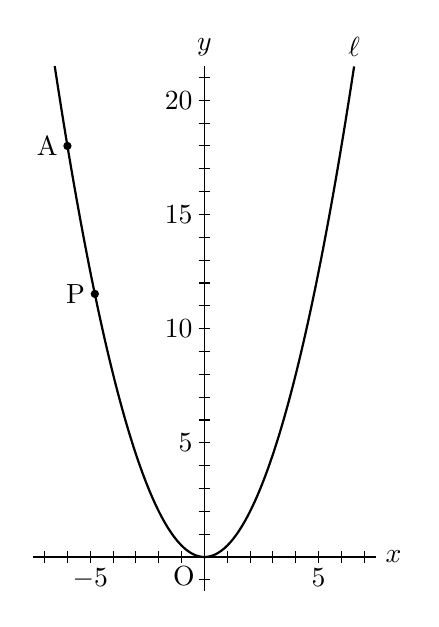
\begin{tikzpicture}[x=2.9mm, y=2.9mm]

    \pgfmathsetmacro{\xmax}{7.5}
    \pgfmathsetmacro{\ymax}{21.5}

    \pgfmathsetmacro{\lxm}{(2*\ymax)^0.5}

    \pgfmathsetmacro{\d}{0.25}

    % 座標軸
    \draw[semithick] (-\xmax,0) -- (\xmax,0) node[right] {$x$};
    \draw[semithick] (0,-1.5) -- (0,\ymax) node[above] {$y$};
    
    % x軸・y軸の目盛り
    \foreach \x in {-7,-6,...,7} {
        \draw (\x,-\d) -- (\x,\d);
    }
    \foreach \y in {-1,0,...,21} {
        \draw (-\d,\y) -- (\d,\y);
    }
    \foreach \x in {-5,5} {
        \node[below, outer sep=1pt] at (\x,0) {$\x$};
    }
    \foreach \y in {5,10,15,20} {
        \node[left, outer sep=1pt] at (0,\y) {$\y$};
    }

    % y=0.5x^2のグラフ
    \draw[thick, domain=-\lxm:\lxm, samples=200] plot (\x,{0.5*\x*\x})
        node[above]{$\ell$};

    % 原点
    \node[below left] at (0,0) {$\mathrm{O}$};
    
    % 点A (-6, 18)
    \fill (-6,18) circle (1.5pt) node[left] {$\mathrm{A}$};

    % 点P (-4.8, 11.52)
    \fill (-4.8,11.52) circle (1.5pt) node[left] {$\mathrm{P}$};
   
\end{tikzpicture}
\end{document}

